%% Revealed-Preference Discount Rates — job talk skeleton (75–90 min)
%% Style: FSIL_slides_Hall_Jul21.tex conventions (Shapiro + paulgp/beamer-tips)
%% Compile: tectonic job_talk.tex   (from Slides/)
%% Placeholders are marked [PLACEHOLDER: ...] in alert orange — pending PACE runs.

\documentclass[11pt,aspectratio=169]{beamer}

\usetheme{default}
\usecolortheme{seagull}
\usepackage{booktabs}
\usepackage{graphicx}
\usepackage{amsmath,amssymb}
\usepackage{xcolor}

\definecolor{gtnavy}{RGB}{0,48,87}
\definecolor{gtgold}{RGB}{179,163,105}
\definecolor{alertorange}{RGB}{213,94,0}
\definecolor{cbblue}{RGB}{0,114,178}
\definecolor{dimgray}{RGB}{150,150,150}
\definecolor{sand}{RGB}{247,243,232}

\setbeamercolor{frametitle}{fg=gtnavy}
\setbeamercolor{title}{fg=gtnavy}
\setbeamercolor{structure}{fg=gtnavy}
\setbeamercolor{alerted text}{fg=alertorange}
\setbeamercolor{button}{bg=white,fg=cbblue}
\setbeamertemplate{navigation symbols}{}
\setbeamertemplate{itemize item}{\textcolor{gtgold}{\small$\blacktriangleright$}}
\setbeamertemplate{itemize subitem}{\textcolor{gtgold}{\scriptsize$\triangleright$}}
\setbeamerfont{frametitle}{series=\bfseries,size=\large}

\newcommand{\fsilsec}{}
\setbeamertemplate{footline}{%
  \hspace{2ex}\scriptsize\textcolor{dimgray}{\fsilsec}%
  \hfill\scriptsize\textcolor{dimgray}{\insertframenumber\,/\,\inserttotalframenumber}\hspace{2ex}\vspace{1ex}}

\newenvironment{wideitemize}{\begin{itemize}\setlength{\itemsep}{0.7em}}{\end{itemize}}
\newcommand{\ph}[1]{\alert{[PLACEHOLDER: #1]}}
\newcommand{\goto}[2]{\hyperlink{#1}{\beamergotobutton{#2}}}
\newcommand{\back}[2]{\hyperlink{#1}{\beamerreturnbutton{#2}}}
\newcommand{\buttonrow}[1]{\vspace{0.3em}\hfill #1}

\newcommand{\rmentry}[3]{\ifnum#1=#2 {\color{gtnavy}\textbf{#3}}\else{\color{dimgray}#3}\fi}
\newcommand{\roadmapframe}[1]{%
{\setbeamercolor{background canvas}{bg=sand}%
\begin{frame}{Roadmap}
  \Large
  \begin{enumerate}
    \item[\rmentry{#1}{1}{1.}] \rmentry{#1}{1}{The question and the data}
    \item[\rmentry{#1}{2}{2.}] \rmentry{#1}{2}{A sufficient statistic for the discount rate}
    \item[\rmentry{#1}{3}{3.}] \rmentry{#1}{3}{Baseline estimates --- and every reason not to believe them, addressed}
    \item[\rmentry{#1}{4}{4.}] \rmentry{#1}{4}{Heterogeneity: who discounts, where, and when}
    \item[\rmentry{#1}{5}{5.}] \rmentry{#1}{5}{Aggregation and what it means}
  \end{enumerate}
\end{frame}}}

\title{\textbf{What Do Defaults Tell Us About Discount Rates?\\
Revealed Preference from 20 Years of Credit-Bureau Data}}
\author{Joseph Hall\\[2pt] \small Georgia Institute of Technology}
\institute{Job Talk}
\date{2026--27 Market}

\begin{document}

\begin{frame}[plain]\titlepage\end{frame}

%% ═══════════════ 1. QUESTION AND DATA ═══════════════
\renewcommand{\fsilsec}{1. Question and data}
\roadmapframe{1}

\begin{frame}{The discount rate is the primitive of household finance}
\begin{wideitemize}
  \item Every intertemporal decision a household makes --- saving, borrowing,
        defaulting, refinancing, retiring --- is priced off one parameter
  \item Yet we mostly measure it by \alert{asking hypothetical questions}
        (elicited rates: 30--100\%+, unstable) or by structural estimation
        inside heavily parameterized models
  \item This paper: measure it from \alert{what borrowers actually do at the
        highest-stakes margin they face} --- default
\end{wideitemize}
\end{frame}

\begin{frame}{Default is an intertemporal trade}
\begin{wideitemize}
  \item A borrower who defaults \alert{keeps the remaining payments} (money
        today and tomorrow) and \alert{accepts the consequences} (chargeoff,
        collections, credit exclusion --- money later)
  \item Where the borrower stops paying therefore \emph{reveals} the rate at
        which they trade the future for the present
  \item The paper turns this observation into a sufficient statistic that
        needs no structural model of the household
\end{wideitemize}
\end{frame}

\begin{frame}{Preview of answers}
\begin{wideitemize}
  \item Revealed-preference annual discount rate: \alert{$\approx 27\%$}
        at the three-year horizon ($\widehat\beta = 0.787$, s.e.\ 0.003) ---
        and the marginal-utility correction is \emph{measured} to be nil
  \item An order of magnitude above risk-free rates; far below elicited rates;
        consistent with behavior in the credit-card literature
  \item The heterogeneity is the economics: rates decline monotonically in
        credit score (26.7\% $\to$ 23.2\%) and in income (25.8\% $\to$
        21.8\%); geography spreads $\beta$ across $[0.73, 0.84]$
  \item And the headline twist: different loan horizons trace out a
        \alert{steeply declining discount curve} --- within person --- a
        discount rate schedule
\end{wideitemize}
\end{frame}

\begin{frame}{The data: the best you could ask for on this question}
\begin{wideitemize}
  \item \textbf{Equifax ACRO archive, 10\% sample of US credit files}:
        every trade line, \alert{monthly snapshots 2005--2024} (240 archives)
  \item Auto loans: \alert{6.2 million} fixed-term loans,
        \alert{277{,}026 defaults} usable for estimation, all 48 continental
        states + DC
  \item Same archive, same estimator, three more contract families:
        \alert{58M first mortgages, 4.9M home-equity, 72M personal
        installment} --- horizons from under two years to seventeen
  \item Terms, payments, balances, chargeoffs, timing --- everything the
        estimator needs, at population scale, for 20 years
\end{wideitemize}
\end{frame}

\begin{frame}{Contribution relative to three literatures}
\begin{wideitemize}
  \item \textbf{Measured discount rates} (elicitation, field experiments):
        we replace stated choices with consequential ones, at 6M-loan scale
  \item \textbf{Consumer default} (strategic default, liquidity default):
        we use default \emph{timing} as information about preferences,
        not just a cost to be explained
  \item \textbf{Household finance measurement} (payment targeting,
        bureau-data methods): we contribute a practitioner's toolkit ---
        rate imputation from quantity fields, power-preserving sample
        design --- reusable beyond this paper
\end{wideitemize}
\end{frame}

%% ═══════════════ 2. THEORY ═══════════════
\renewcommand{\fsilsec}{2. Sufficient statistic}
\roadmapframe{2}

\begin{frame}{Two periods, one identity}
\begin{wideitemize}
  \item Defaulting borrower keeps remaining payments $A$, loses chargeoff
        consequences $B$, with continuation default risk $p_2$
  \item Indifference at the observed stopping point delivers the
        \alert{exact identity}
        \[ \frac{A}{(1-p_2)\,B + A} \;=\; \beta\,\lambda \]
  \item $\beta$: the discount factor. $\lambda$: relative marginal utility of
        the default state --- the correction term the literature usually
        assumes away
\end{wideitemize}
\end{frame}

\begin{frame}{From identity to estimator}
\begin{wideitemize}
  \item Implementation: two fixed-effects logits (default on log payment;
        default on log total obligation) within score-ventile
        $\times$ zip-by-month cells
  \item $\widehat{R} = \widehat{\gamma}_L / (\widehat{\gamma}_L +
        \widehat{\gamma}_m)$, annualized through mean defaulter horizon
        $\widehat{\Delta T}$:
        \[ \widehat{\beta} \;=\; \widehat{R}^{\,1/\widehat{\Delta T}} \]
  \item Identification: cross-sectional variation in payment size against
        obligation size, within cells that absorb local shocks and
        creditworthiness
\end{wideitemize}
\end{frame}

\begin{frame}{The theory extends as far as anyone will push it}
\begin{wideitemize}
  \item $T$-period and continuous-time generalizations: the identity survives
        as the envelope condition of the optimal stopping problem
        (Appendix; available for the whiteboard)
  \item Heterogeneous agents: aggregation theory for what a population
        $\beta$ distribution implies for measured aggregates ---
        pooled estimation recovers a sensitivity-weighted average of
        type-level statistics (exact aggregation proposition)
  \item Marginal-utility correction: \alert{measured directly in the panel} ---
        the key input is the persistence of the marginal borrower's state,
        and 21.4M delinquency transitions put it at $\rho = 0.992$
        $\Rightarrow$ $\lambda = 1.00$, correction nil (the literature's
        lower-persistence calibrations move the rate to no less than 25\%)
\end{wideitemize}
\end{frame}

%% ═══════════════ 3. BASELINE + CREDIBILITY ═══════════════
\renewcommand{\fsilsec}{3. Baseline and credibility}
\roadmapframe{3}

\begin{frame}[label=baseline]{Baseline estimate}
\begin{wideitemize}
  \item $\widehat{\beta} = 0.787$ (s.e.\ 0.003) $\Rightarrow$
        \alert{$\approx 27\%$ per year} at the three-year horizon
  \item The one approximation is measured away: at the panel's own
        distress persistence, $\lambda = 1.00$ --- the correction is nil
  \item And the clock is not doing the work: the sensitivity ratio
        $R = 0.465$ would need $T = 18.8$ years on five-year loans to be
        consistent with $\beta = 0.96$
  \item Benchmarks: risk-free $\sim$2--4\%; credit-card APRs
        $\sim$20--25\%; elicited experimental rates 30--100\%+
\end{wideitemize}
\buttonrow{\goto{b_mu}{measured correction}\ \goto{b_tvr}{is it just $T$?}\ \goto{b_power}{precision}}
\end{frame}

\begin{frame}[label=power]{Power here is a theorem}
\begin{center}
\Large
$\operatorname{se}(\widehat{\beta}) \;=\; \dfrac{c}{\sqrt{n_{\text{defaults}}}}$
\end{center}
\vspace{0.5em}
\begin{wideitemize}
  \item Rare-events information: every entry of the estimator's covariance
        scales with $1/n_d$ --- \alert{loans are free, defaults are power}
  \item Validated on 136 geographic clusters: log-log slope $-0.615$
        $(0.077)$; conditional on defaults, the loan count contributes
        \alert{exactly nothing}: $-0.016$ $(0.153)$
  \item Consequence: every sample split in this paper is designed at the
        default margin (equal-default bands, default-floor clusters)
\end{wideitemize}
\end{frame}

\begin{frame}[label=threat_rate]{Threat 1: ``you never observe the interest rate''}
\begin{wideitemize}
  \item Correct --- no credit bureau records prices; the \texttt{rate} field
        is a payment-status code
  \item Answer: the contract's quantity side $(L, m, T)$ \alert{overidentifies}
        the rate --- annuity inversion at origination, balance-path recovery
        from monthly snapshots
  \item Both validated on simulated bureau data with known rates; the two
        methods fail on \alert{disjoint} reporting quirks, so their agreement
        is a data-quality diagnostic (Appendix: practitioner's guide)
\end{wideitemize}
\buttonrow{\goto{b_impute}{error taxonomy}}
\end{frame}

\begin{frame}[label=threat_endog]{Threat 2: ``payment size is endogenous''}
\begin{wideitemize}
  \item We killed our own first instrument, in public: rate levels at
        origination fail three redesigns (vintage confounding --- a purely
        cohort-level instrument cannot be rescued)
  \item The living design: \alert{lender-menu leniency} --- the staggered
        60$\to$72$\to$84-month term expansion and lender size menus give
        two leave-one-out instruments in the \emph{same} sample as the FE
        strategy; first stages $F = 221$ and $F = 47{,}000$
  \item Where the well-identified designs and the FE specifications
        meet: HAMP RD 0.76, bankruptcy RKD 0.78, and the FE family
        0.79--0.80 across three specifications --- the agreement table
  \item Lender-policy natural experiments are bundled treatments in
        this data (adoption events shift clientele too); the sharpness
        diagnostics and the graveyard are all reported
\end{wideitemize}
\buttonrow{\goto{b_iv}{the instrument graveyard}}
\end{frame}

\begin{frame}[label=threat_sel]{Threat 3: ``defaulters are selected''}
\begin{wideitemize}
  \item Of course --- the estimator \emph{conditions} on the default margin;
        the question is what changes across comparisons
  \item Cross-group comparisons hold the margin fixed by design
        (equal-default bands); geographic correlations are re-estimated
        under default-composition controls
  \item Example below: the income--patience correlation \alert{dies} under the
        selection control; the poverty and partisanship correlations
        \alert{survive} --- the paper reports both honestly
\end{wideitemize}
\buttonrow{\goto{b_select}{full table}}
\end{frame}

\begin{frame}[label=threat_liq]{Threat 4: ``they just can't pay''}
\begin{wideitemize}
  \item \alert{65\% of 2.46M auto defaulters keep paying other creditors}
        six months \emph{after} the chargeoff (10.7 other trades on
        average; only 1.6\% default on everything) --- the modal default is
        a portfolio choice
  \item $\widehat\beta$ is \alert{flat across local labor shocks}:
        0.774 / 0.786 / 0.789 by unemployment-change tercile
  \item The same borrower reveals 29\% on personal loans, 12\% on autos,
        1\% on the mortgage --- \alert{one budget cannot bind selectively}
  \item Distress is measured near-permanent ($\rho = 0.992$) --- the
        transitory-shock story contradicts the data; the permanent-state
        story \emph{is} the measured $\lambda$
\end{wideitemize}
\buttonrow{\goto{b_liq}{Monte Carlo: why $\widehat\beta$ can't acquit itself}}
\end{frame}

\begin{frame}[label=threat_rich]{Threat 5: ``they just expect to be rich''}
\begin{center}
\Large ``Everyone was a temporarily\\[0.2em] embarrassed capitalist.''\\[0.9em]
\normalsize --- John Steinbeck, ``A Primer on the Thirties,'' \emph{Esquire}, 1960\\[0.3em]
{\footnotesize (the popular ``temporarily embarrassed millionaires'' is Ronald Wright's 2004 paraphrase)}
\end{center}
\vspace{0.6em}
\begin{wideitemize}
  \item The objection: high borrowing rates reveal expected income growth,
        not impatience
  \item Three answers, in increasing strength: distress at the default
        margin is measured near-permanent ($\rho = 0.99$, 0.26\% of
        spells cure per quarter); the growth calibrations large enough to
        matter are refuted by the data's own bound ($\lambda \ge 0.47$);
        and the SCF lower bounds hand every household its \emph{most
        optimistic} lifecycle income path --- the 16--20\% floor survives
  \item Even a temporarily embarrassed capitalist should not pay 25\%
        APR once the model has priced in the capital
\end{wideitemize}
\end{frame}

%% ═══════════════ 4. HETEROGENEITY ═══════════════
\renewcommand{\fsilsec}{4. Heterogeneity}
\roadmapframe{4}

\begin{frame}{The economics lives in the cross-section of $\beta$}
\begin{wideitemize}
  \item A single aggregate discount rate answers no policy question ---
        \alert{who} is impatient governs the incidence of every
        intertemporal policy: moratoria, minimum payments, forbearance,
        retirement defaults
  \item This section: credit score, income, loan type, geography,
        political geography, and time
  \item Power-preserving design: every cell flagged by its default count,
        nothing silently pooled
\end{wideitemize}
\end{frame}

\begin{frame}{By credit score and income: monotone, precise, modest}
\begin{center}
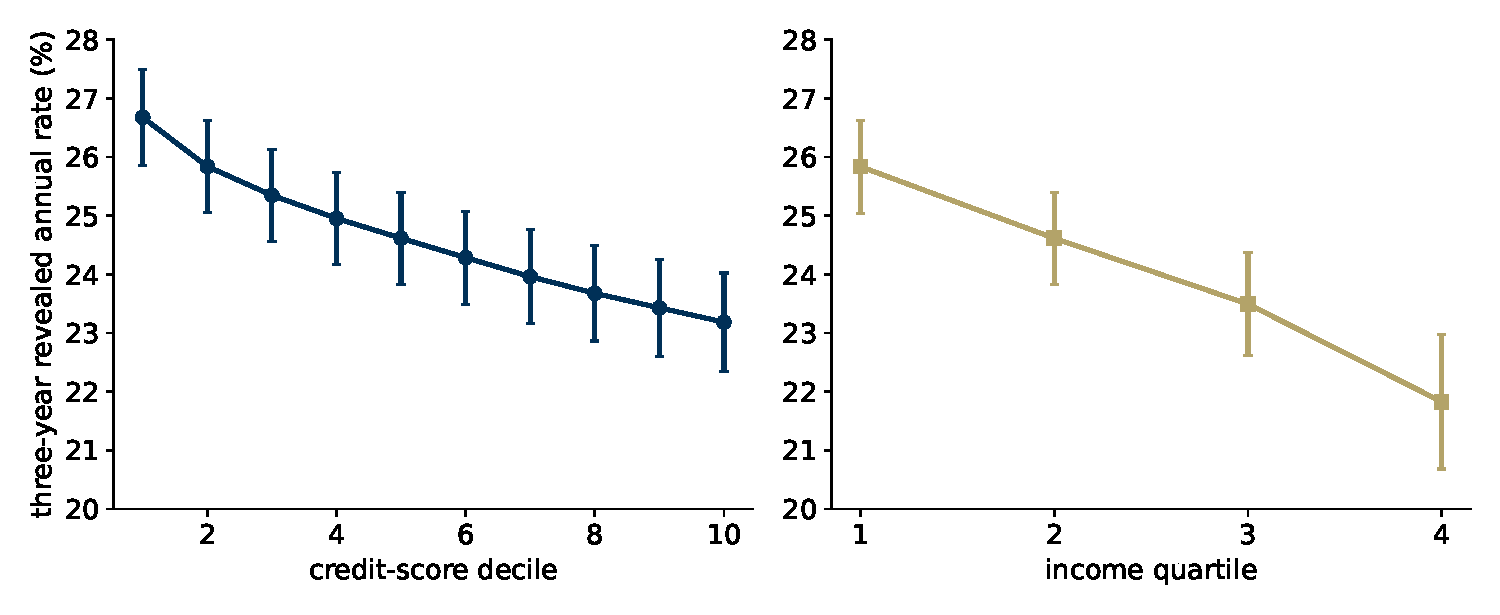
\includegraphics[width=0.86\textwidth]{fig_vc_gradients.pdf}
\end{center}
\vspace{-0.3em}
\small Varying-coefficient design: every default informs every cell, so
the bands are \alert{0.4pp} wide. Both gradients are monotone; both are
modest against the 20--27\% level. High default rates among low-score
borrowers are mostly something other than impatience.
\end{frame}

\begin{frame}[label=curve]{The revealed discount curve, traced loan by loan}
\begin{center}
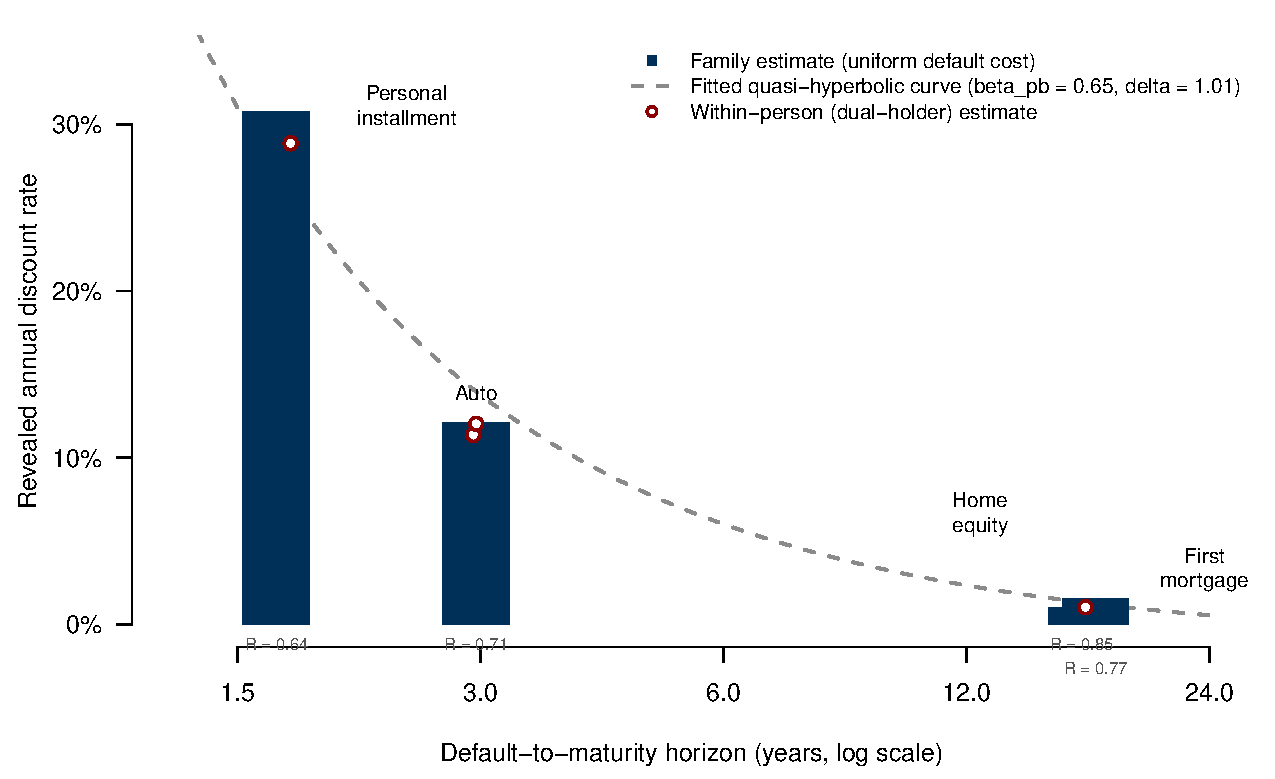
\includegraphics[width=0.78\textwidth]{fig_term_structure.pdf}
\end{center}
\vspace{-0.4em}
\small Four families, one estimator, uniform default cost --- the annual
rate falls from \alert{31\% at a 1.7-year horizon to 1\% at seventeen
years}, and the dual-holder markers show it \alert{within person}.
The measurement is a schedule.
\buttonrow{\goto{b_curve}{$(\beta_{pb}, \delta)$ identification}\ \goto{b_liq}{not liquidity}}
\end{frame}

\begin{frame}{Geography: 136 power-designed clusters, 48 states}
\begin{wideitemize}
  \item Sub-state clusters built on zip3 adjacency to a default floor;
        estimated cluster-by-cluster with the full estimator
  \item Cross-cluster spread is \alert{large}: $\beta$ p10--p90
        $[0.733, 0.835]$ --- annual rates from $\sim$20\% to $\sim$36\%
  \item Decomposition: 84\% of the cross-cluster variance in
        $\log\beta$ comes from the default sensitivities alone; the
        horizon contributes 2\%
\end{wideitemize}
\end{frame}

\begin{frame}{What geography correlates with}
\begin{wideitemize}
  \item Merged with IRS SOI zip3 covariates (loan-count weighted):
  \item \alert{Poverty (EITC share): $\rho_w = -0.37$}, slope $-0.42$
        $(0.09)$ --- poorer areas show \emph{lower} measured discount rates;
        survives default-composition control
  \item Income level: raw positive, \alert{dies under the selection control}
        --- reported as a selection artifact
  \item Unemployment share, itemizer share: positive, state-FE fragile
\end{wideitemize}
\end{frame}

\begin{frame}{Political geography: patience leans Republican}
\begin{wideitemize}
  \item County presidential returns (2008--2024) crosswalked to clusters
  \item 2020 GOP two-party share: $\rho_w = -0.19$ (Spearman $-0.30$);
        slope $-0.088$ $(0.040)$, \alert{strengthens} under the
        default-composition control ($-0.101$ $(0.038)$)
  \item The 2016--2020 \alert{swing is a precise zero} ($\rho_w = 0.01$) ---
        the partisan \emph{level} correlates with patience; the Trump-era
        movement is orthogonal to it
  \item Five-cycle panel (2008--2024) in estimation \ph{geography $\times$
        cycle betas --- within-cluster changes, lead-lag structure}
  \item \textcolor{dimgray}{\footnotesize Companion analysis: enters the
        manuscript with the next estimation cycle; replication outputs in
        the project repository}
\end{wideitemize}
\end{frame}

\begin{frame}{Across time: patience is rising}
\begin{wideitemize}
  \item State $\times$ cycle cells, five presidential cycles: median
        $\beta$ climbs \alert{0.719 $\to$ 0.764 $\to$ 0.779 $\to$ 0.774
        $\to$ 0.808} from 2005--08 to 2021--24
  \item Rates at the default margin fell from $\sim$39\% to $\sim$24\%
        over two decades --- composition, credit access, or preference
        drift: the panel can ask
  \item Recession cohorts run more impatient (0.731 vs.\ 0.792) ---
        a composition effect the paper flags and does not over-read
\end{wideitemize}
\end{frame}

%% ═══════════════ 5. AGGREGATION AND MEANING ═══════════════
\renewcommand{\fsilsec}{5. Aggregation and meaning}
\roadmapframe{5}

\begin{frame}{From micro $\beta$ to macro objects}
\begin{wideitemize}
  \item Heterogeneous-agents aggregation: measured aggregates load on the
        \emph{patient tail}, so population medians and macro calibrations
        answer different questions
  \item The 27\% median coexists with standard macro calibrations, and
        the aggregation proposition states exactly how
\end{wideitemize}
\end{frame}

\begin{frame}{What it means}
\begin{wideitemize}
  \item Incidence: debt relief and forbearance are transfers \emph{to} the
        impatient margin, and the margin is now measured
  \item Pricing: lenders setting minimum payments face a distribution of
        $\beta$ this paper measures directly
  \item Measurement: the toolkit (rate imputation, power-preserving splits,
        the exact identity) transfers to any bureau-data setting
\end{wideitemize}
\end{frame}

\begin{frame}{Conclusion}
\begin{wideitemize}
  \item Defaults reveal discount rates: \alert{$\approx$27\%/year} at the
        three-year horizon --- and a \alert{steeply declining schedule}
        across horizons, within person
  \item The best available data, attacked with an exact identity, a
        \emph{measured} correction, designed power, and every objection
        diagnosed in the open
  \item The discount curve (four bars, one dashed line) is the picture to
        leave the room with \goto{curve}{the curve}
\end{wideitemize}
\end{frame}

%% ═══════════════ BACKUP ARSENAL ═══════════════
\renewcommand{\fsilsec}{Backup}
{\setbeamercolor{background canvas}{bg=sand}%
\begin{frame}{Backup arsenal}
\small Organized for the fight: theory, calibration, power, imputation,
selection, data plumbing.
\end{frame}}

\begin{frame}{Backup: exact identity, full derivation}
\begin{wideitemize}
  \item Two periods: implicit differentiation of the period-1 threshold
        gives $\partial p_1/\partial L = f(y_1^*)\beta(1-p_2)
        \mathbb{E}[u'(C_2^P)\mid y_2 > y_2^*]/\Delta u_1'$ and
        $\partial p_1/\partial m$ as the current-payment analogue
  \item The ratio cancels the margin density and the utility scale,
        leaving $\beta\lambda$
  \item $T$ periods: the same identity survives as the envelope condition
        of optimal stopping, provided the punishment has a flow component
        and good standing carries the option to default later
\end{wideitemize}
\end{frame}

\begin{frame}{Backup: continuous-time statement}
\begin{wideitemize}
  \item Continuous time: default is a stopping time on the income process,
        and the identity appears as the smooth-pasting condition at the
        default boundary
  \item The response of stopping to a payment perturbation at horizon $s$
        is $D(s)$ times the survival-weighted marginal utility at $s$ ---
        ratios across horizons identify the discount function
        nonparametrically
  \item Two horizons point-identify quasi-hyperbolic $(\beta_{pb},
        \delta)$; three make the exponential null testable
\end{wideitemize}
\end{frame}

\begin{frame}[label=b_mu]{Backup: the marginal-utility correction, measured}
\begin{wideitemize}
  \item The key input is the persistence of the marginal borrower's state:
        21{,}350{,}801 delinquency-spell transitions, \alert{0.26\% cure
        per quarter} $\Rightarrow$ $\rho = 0.992$ annualized
  \item At measured $\rho$: $\lambda = 1.00$ at the
        Blundell--Pistaferri--Preston pass-through --- \alert{correction
        nil}; the headline stands as measured
  \item Literature-persistence sensitivity ($\rho = 0.95$, STY 2004):
        $\lambda = 0.95$, corrected rate 25\% --- the floor across every
        admissible calibration
  \item Internal-consistency bound: identification requires
        $\lambda \ge \widehat\beta^{\,T} = 0.47$, refuting exactly the
        calibrations that would generate large corrections
\end{wideitemize}
\buttonrow{\back{baseline}{back: baseline}}
\end{frame}

\begin{frame}[label=b_tvr]{Backup: the clock contributes little}
\begin{wideitemize}
  \item Decompose cross-group variance of $\log\beta$ into sensitivity
        ($R$) and horizon ($T$) contributions: geography \alert{84\%
        $R$-only} (rank correlation 0.97 at fixed $T$); state-cycle 89\%
  \item Levels are $T$-proof: $R = 0.465$ requires \alert{$T = 18.8$
        years on five-year loans} to be consistent with $\beta = 0.96$;
        a 20\% error in $T$ moves the headline 27\% $\to$ 22\%
  \item Where $T$ \emph{does} carry magnitude --- across loan families ---
        that is the term-structure result, promoted to a finding
\end{wideitemize}
\buttonrow{\back{baseline}{back: baseline}\ \back{curve}{back: the curve}}
\end{frame}

\begin{frame}[label=b_liq]{Backup: the estimator under liquidity-driven default}
\begin{wideitemize}
  \item Ground rule: in a simulated pure-liquidity economy,
        $\widehat\beta$ lands at \alert{0.78, not 0} --- obligations load
        mechanically on payments, so $\widehat\beta$ alone cannot referee
  \item Mixture path (true $\beta = 0.95$): $\widehat\beta$ falls
        0.887 $\to$ 0.783 as the liquidity share goes $0 \to 1$
  \item Default-rate-matched surface, true $\beta \in [0.55, 0.99]$
        $\times$ shares up to 0.50: \alert{no cell reaches the measured
        0.787} --- patient preferences plus admissible contamination
        cannot manufacture the estimate
\end{wideitemize}
\buttonrow{\back{threat_liq}{back: threat 4}\ \back{curve}{back: the curve}}
\end{frame}

\begin{frame}[label=b_curve]{Backup: two horizons identify $(\beta_{pb}, \delta)$}
\begin{wideitemize}
  \item Quasi-hyperbolic $D(t) = \beta_{pb}\,\delta^{t}$: with horizon
        factors $b(T) = D(T)^{1/T}$,
        $\ln\beta_{pb} = \dfrac{\ln b(T_1) - \ln b(T_2)}{1/T_1 - 1/T_2}$
  \item Dual holders: auto $\times$ mortgage $\Rightarrow$
        $\beta_{pb} = 0.71$, $\delta = 1.01$; auto $\times$ personal
        $\Rightarrow$ $\beta_{pb} = 0.55$, $\delta = 1.09$ ---
        \alert{large present bias, long-run rate $\approx$ 0} within
        measurement error
  \item Estimand discipline: every cross-person object is
        \emph{horizon-labeled}; cross-horizon statements are statements
        about the curve; the schedule-proof heterogeneity object is the
        joint distribution of $(\beta_{pb}, \delta)$
\end{wideitemize}
\buttonrow{\back{curve}{back: the curve}}
\end{frame}

\begin{frame}[label=b_power]{Backup: power law --- matrix statement}
\[ \operatorname{Avar}(\widehat{\beta}) = \nabla g' \, \Sigma \, \nabla g,
\qquad \Sigma = V / n_d, \qquad
\mathcal{I}(\gamma) \approx \mathbb{E}[n_d] \cdot M \]
\begin{wideitemize}
  \item Rare-events logit information proportional to expected events
        (King--Zeng 2001); $M$ = default-weighted design moment
  \item Horse race across 136 clusters: $\ln n_d$ coefficient $-0.608$
        $(0.102)$; $\ln n$ coefficient $-0.016$ $(0.153)$
\end{wideitemize}
\buttonrow{\back{baseline}{back: baseline}}
\end{frame}

\begin{frame}[label=b_impute]{Backup: rate imputation --- error taxonomy}
\begin{wideitemize}
  \item Method 1 exact except: odd first period ($+18$bp), balloons
        (adjusted inversion restores exactness)
  \item Method 2 exact except intermittent stale balances ($-0.1$bp median
        rule) and curtailments ($-0.6$bp median; mean version explodes)
  \item Financed fees: no bias; a $\sim$77bp note-rate/APR wedge at 2\% fees
        --- imputed rates lower-bound Reg-Z APRs
\end{wideitemize}
\buttonrow{\back{threat_rate}{back: threat 1}}
\end{frame}

\begin{frame}[label=b_select]{Backup: selection diagnostics, full table}
\begin{wideitemize}
  \item Poverty (EITC share): slope $-0.42$ $(0.09)$ without the
        default-composition control, and the correlation survives with it
  \item Zip-level income: positive in the raw cross-section and gone
        under the control --- reported as a selection artifact
  \item Partisanship level: $-0.088$ $(0.040)$ raw, $-0.101$ $(0.038)$
        controlled; the 2016--2020 swing is a precise zero
\end{wideitemize}
\buttonrow{\back{threat_sel}{back: threat 3}}
\end{frame}

\begin{frame}[label=b_iv]{Backup: the instrument graveyard, and the living design}
\begin{wideitemize}
  \item GS3-at-origination, three repairs, three failures: vintage
        controls ($\beta = 1.14$, CF $= 4.7$), AR(1) innovations
        (first-stage $F = 0.0$), imputed-rate target ($\beta = 1.07$) ---
        a purely cohort-level instrument cannot be rescued
  \item Menu leniency: first stages $F_{dur} = 221$, $F_{size} = 47{,}288$
        (lender-clustered); naive CF flips $\gamma_m$ --- long-term-menu
        lenders are subprime, menus proxy clientele
  \item Lender-FE iteration: within-lender instrument too weak for the
        control function --- recorded; the agreement exhibit rests on the
        external designs and FE spec stability
\end{wideitemize}
\buttonrow{\back{threat_endog}{back: threat 2}}
\end{frame}

\begin{frame}{Backup: data plumbing that survives review}
\begin{wideitemize}
  \item Single deterministic pipeline, fail-fast probes, restartable
        extracts; every exhibit regenerated from raw archives
  \item Known traps handled: zip zero-padding, integer overflow in
        population-weighted merges, CT's 2024 FIPS redistricting,
        left-truncated pre-2005 cohorts, censored 2021+ cohorts
\end{wideitemize}
\end{frame}

\begin{frame}{Backup: what the archive contains}
\begin{wideitemize}
  \item 73 fields per trade-month; flags for every loan family; balloon,
        deferral, and narrative codes (fixed vs.\ variable rate)
  \item 240 monthly archives $\times$ 10\% of US credit files, 2005--2024
\end{wideitemize}
\end{frame}

\end{document}
